\section{Investimento da parte del gruppo}
	\subsection{Dettaglio fasi}
		\subsubsection{Fase A}
			\paragraph{Suddivisione lavoro}
				Nella \insphase{Fase A} ogni componente del gruppo \groupname{} coprirà i seguenti ruoli:
				\begin{table}[H]
					\begin{center}
						\begin{tabular}{| l | c | c | c | c | c | c | c |}
							\hline
							Componente 				& PM	& Am 	& An 	& Pt 		& Pm 	& Ve 	& Ore Totali componente \\ \hline
							
							Bigarella Chiara 			& 0		& 5 		& 30 		& 0		& 0		& 8 		& 43 \\
							Bucco Riccardo 				& 0		& 5 		& 30 		& 0		& 0		& 8 		& 43 \\
							Carlon Chiara	 			& 0		& 6 		& 9 		& 0		& 0		& 17 		& 32 \\
							Dal Bianco Davide 			& 0		& 14 		& 25 		& 0		& 0		& 5 		& 44 \\
							Moretto Alessandro 			& 25 	& 0			& 9 		& 0		& 0		& 8 		& 42 \\
							Pavanello Fabio Matteo	 	& 0		& 5 		& 6 		& 0		& 0		& 23 		& 34 \\
							Rubin Marco					& 7 	& 19 		& 0			& 0		& 0		& 8 		& 34 \\ \hline \hline
							
							Ore Totali Ruolo 			& 32 	& 54 		& 109 		& 0		& 0		& 77 		& 272\\ \hline
						\end{tabular}
					\end{center}
					\caption{Suddivisione ore di lavoro Fase A}
				\end{table}
				Riassumendo con un Bar Chart:
				\begin{figure}[H]\centering
					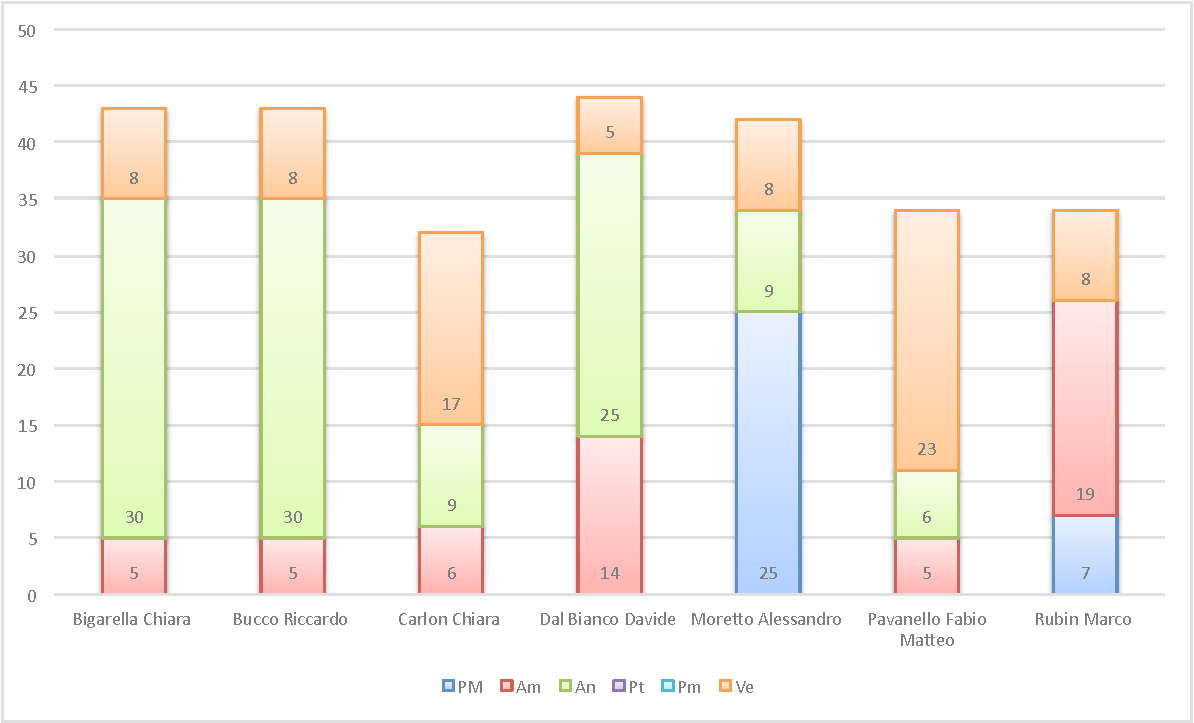
\includegraphics[width=\textwidth]{PianoDiProgetto/Pics/ChartOreFaseA.pdf}
					\caption{Bar Chart ore persona Fase A}
				\end{figure}
			\paragraph{Prospetto economico}
				Nella \insphase{Fase A} il costo di ogni ruolo è il seguente:
				\begin{table}[H]
					\begin{center}
						\begin{tabular}{| l | c | c |}
							\hline
							Ruolo 			& Ore 	& Costi  \\ \hline
							
							Project Manager	& 32 			& \euro{} 960,00 	\\
							Amministratore 		& 54 		& \euro{} 1~080,00 	\\
							Analista	 		& 109 		& \euro{} 2~725,00 	\\
							Progettista 		& 0			& \euro{} 0,00 	\\
							Programmatore		& 0			& \euro{} 0,00	\\
							Verificatore		& 77 		& \euro{} 1~155,00 	\\ \hline \hline
							
							Totale	 		& 272 	& \euro{} 5~920,00 	\\ \hline
						\end{tabular}
					\end{center}
					\caption{Costi per ruolo Fase A}
				\end{table}
				Riassumendo le ore per ruolo con un Pie Chart:
				\begin{figure}[H]\centering
					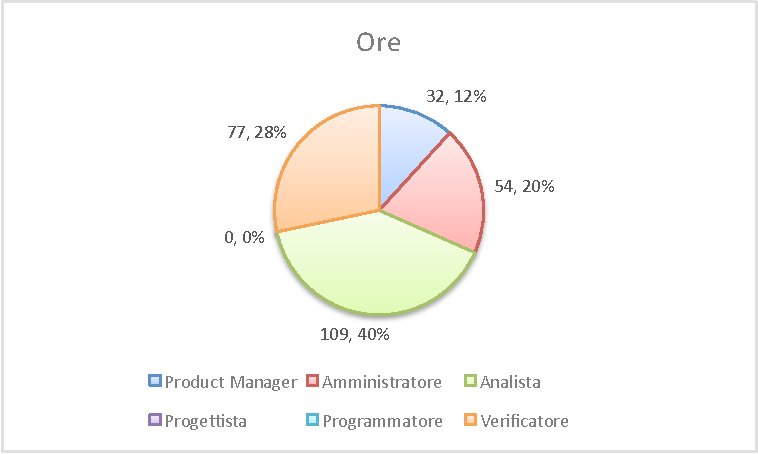
\includegraphics[width=\textwidth]{PianoDiProgetto/Pics/ChartTotOreFaseA.pdf}
					\caption{Pie Chart ore per ruolo Fase A}
				\end{figure}
				Riassumendo i costi per ruolo con un Pie Chart:
				\begin{figure}[H]\centering
					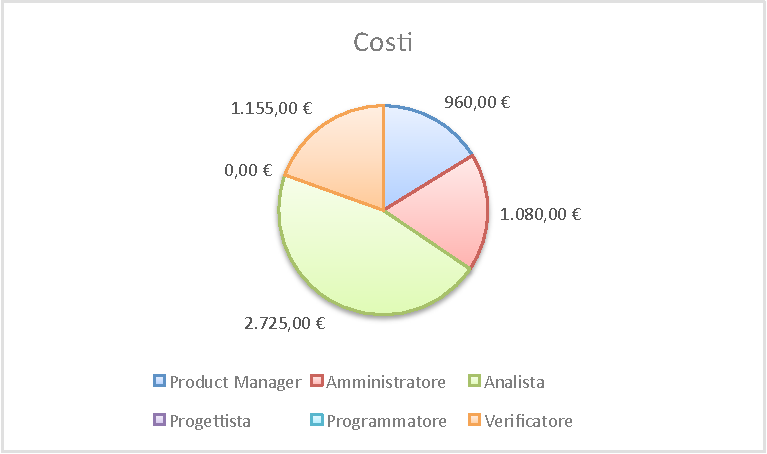
\includegraphics[width=\textwidth]{PianoDiProgetto/Pics/ChartTotCostiFaseA.pdf}
					\caption{Pie Chart costi per ruolo Fase A}
				\end{figure}
		\subsubsection{Fase AD}
			\paragraph{Suddivisione lavoro}
				Nella \insphase{Fase AD} ogni componente del gruppo \groupname{} coprirà i seguenti ruoli:
				\begin{table}[H]
					\begin{center}
						\begin{tabular}{| l | c | c | c | c | c | c | c |}
							\hline
							Componente 				& PM	& Am 	& An 	& Pt 		& Pm 	& Ve 	& Ore Totali componente \\ \hline
							
							Bigarella Chiara 			& 0		& 7 		& 0		& 0		& 0		& 5 		& 12 \\
							Bucco Riccardo 			& 0		& 6 		& 0		& 0		& 0		& 7 		& 13 \\
							Carlon Chiara	 			& 7 		& 0		& 3 		& 0		& 0		& 2 		& 12 \\
							Dal Bianco Davide 			& 0		& 6 		& 0		& 0		& 0		& 5 		& 11 \\
							Moretto Alessandro 			& 0		& 0		& 3 		& 0		& 0		& 8 		& 11 \\
							Pavanello Fabio Matteo	 	& 0		& 0		& 3 		& 0		& 0		& 10 		& 13 \\
							Rubin Marco				& 0		& 0		& 3 		& 0		& 0		& 10 		& 13 \\ \hline \hline
							
							Ore Totali Ruolo 			& 7 		& 19 		& 12 		& 0		& 0		& 47 		& 85\\ \hline
						\end{tabular}
					\end{center}
					\caption{Suddivisione ore di lavoro Fase AD}
				\end{table}
				Riassumendo con un Bar Chart:
				\begin{figure}[H]\centering
					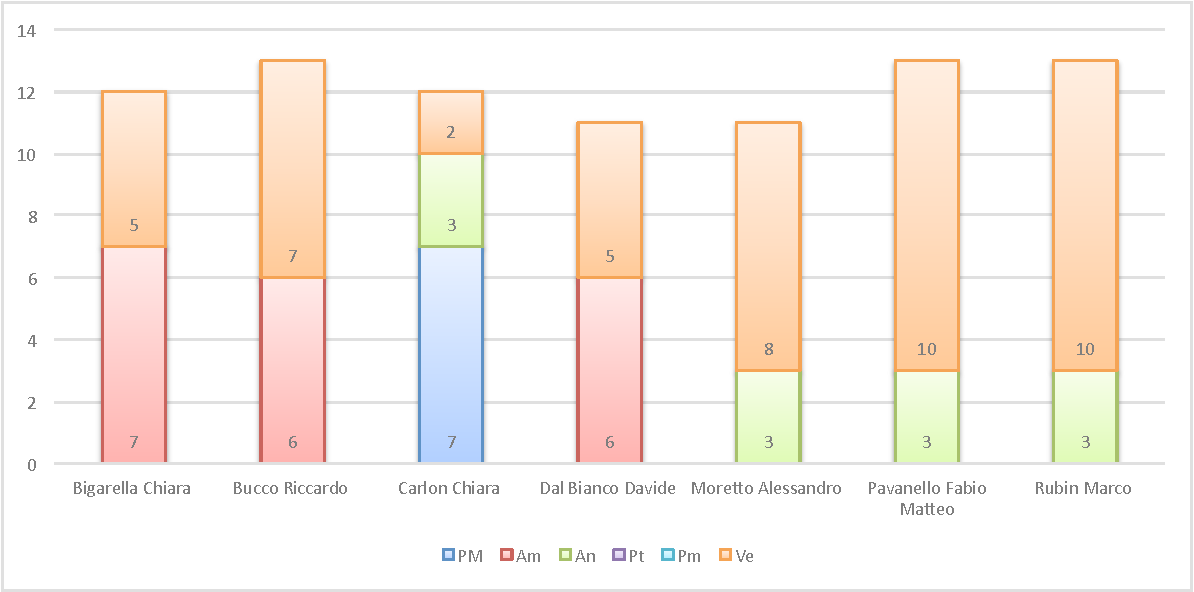
\includegraphics[width=\textwidth]{PianoDiProgetto/Pics/ChartOreFaseAD.pdf}
					\caption{Bar Chart ore persona Fase AD}
				\end{figure}
			\paragraph{Prospetto economico}
				Nella \insphase{Fase AD} il costo di ogni ruolo è il seguente:
				\begin{table}[H]
					\begin{center}
						\begin{tabular}{| l | c | c |}
							\hline
							Ruolo 			& Ore 	& Costi  \\ \hline
							
							Project Manager	& 7 		& \euro{} 210,00 	\\
							Amministratore 		& 19 		& \euro{} 380,00 	\\
							Analista	 		& 12 		& \euro{} 300,00 	\\
							Progettista 		& 0		& \euro{} 0,00 	\\
							Programmatore		& 0		& \euro{} 0,00	\\
							Verificatore		& 47 		& \euro{} 705,00 	\\ \hline \hline
							
							Totale	 		& 85 		& \euro{} 1~595,00 	\\ \hline
						\end{tabular}
					\end{center}
					\caption{Costi per ruolo Fase AD}
				\end{table}
				Riassumendo le ore per ruolo con un Pie Chart:
				\begin{figure}[H]\centering
					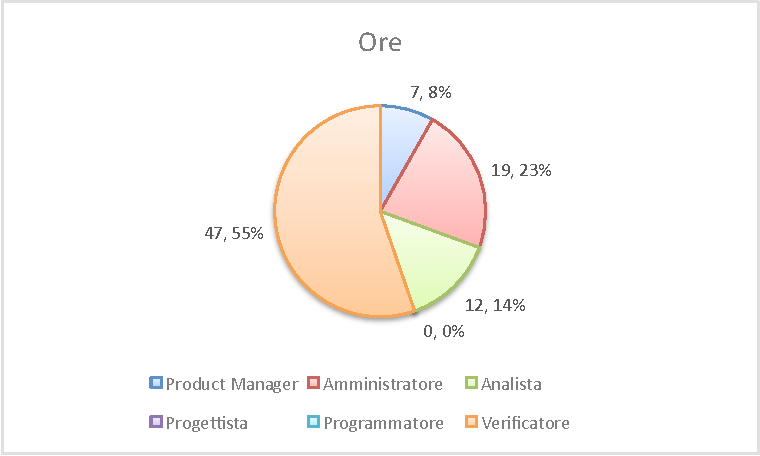
\includegraphics[width=\textwidth]{PianoDiProgetto/Pics/ChartTotOreFaseAD.pdf}
					\caption{Pie Chart ore per ruolo Fase AD}
				\end{figure}
				Riassumendo i costi per ruolo con un Pie Chart:
				\begin{figure}[H]\centering
					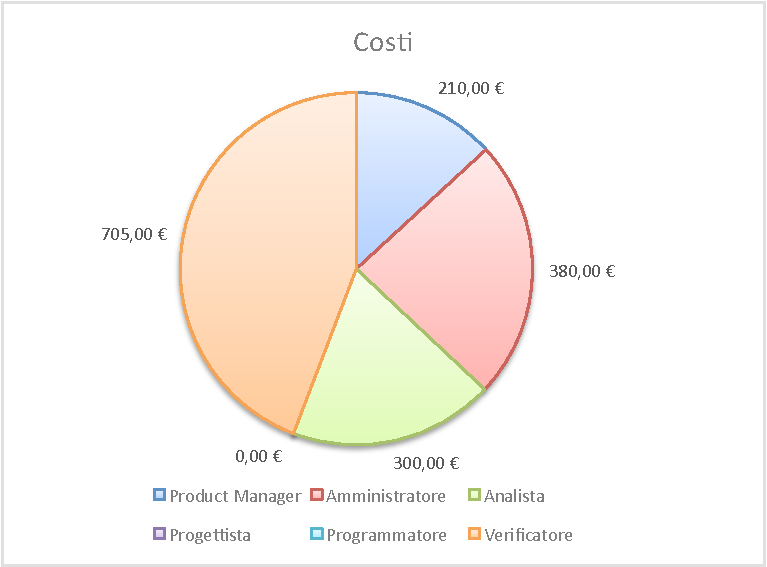
\includegraphics[width=\textwidth]{PianoDiProgetto/Pics/ChartTotCostiFaseAD.pdf}
					\caption{Pie Chart costi per ruolo Fase AD}
				\end{figure}		
	\subsection{Totale}
			\subsubsection{Suddivisione lavoro}
				La suddivisione delle ore di investimento per ruolo di ogni componente del gruppo \groupname{} saranno le seguenti:
				\begin{table}[H]
					\begin{center}
						\begin{tabular}{| l | c | c | c | c | c | c | c |}
							\hline
							Componente 				& PM	& Am 	& An 	& Pt 		& Pm 	& Ve 	& Ore Totali componente \\ \hline
							
							Bigarella Chiara 			& 0		& 12 		& 30 		& 0		& 0		& 13 		& 55 \\
							Bucco Riccardo 				& 0		& 11 		& 30 		& 0		& 0		& 15 		& 56 \\
							Carlon Chiara	 			& 7 	& 6 		& 12 		& 0		& 0		& 19 		& 44 \\
							Dal Bianco Davide 			& 0		& 20 		& 25 		& 0		& 0		& 10 		& 55 \\
							Moretto Alessandro 			& 25 	& 0			& 12 		& 0		& 0		& 16 		& 53 \\
							Pavanello Fabio Matteo	 	& 0		& 5 		& 9 		& 0		& 0		& 33 		& 47 \\
							Rubin Marco					& 7 	& 19 		& 3 		& 0		& 0		& 18 		& 47 \\ \hline \hline
							
							Ore Totali Ruolo 			& 39 	& 73 		& 121	 	& 0		& 0		& 124 		& 357\\ \hline
						\end{tabular}
					\end{center}
					\caption{Suddivisione ore totali di investimento}
				\end{table}
				Riassumendo con un Bar Chart:
				\begin{figure}[H]\centering
					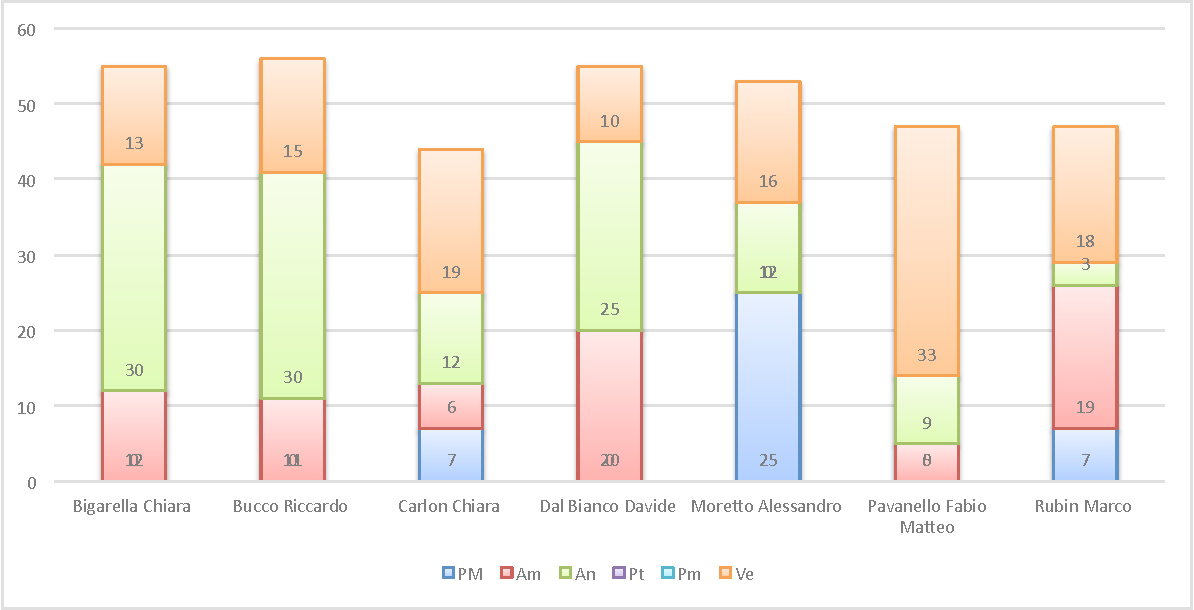
\includegraphics[width=\textwidth]{PianoDiProgetto/Pics/ChartOreInvest.pdf}
					\caption{Bar Chart ore totali di investimento}
				\end{figure}
			\subsubsection{Prospetto economico}
				L'investimento per ogni ruolo è il seguente:
				\begin{table}[H]
					\begin{center}
						\begin{tabular}{| l | c | c |}
							\hline
							Ruolo 			& Ore 		& Costi  \\ \hline
							
							Project Manager	& 39 		& \euro{} 1~170,00 	\\
							Amministratore 		& 73 		& \euro{} 1~460,00 	\\
							Analista	 		& 121 	& \euro{} 3~025,00 	\\
							Progettista 		& 0		& \euro{} 0,00 	\\
							Programmatore		& 0		& \euro{} 0,00	\\
							Verificatore		& 124 	& \euro{} 1~860,00 	\\ \hline \hline
							
							Totale	 		& 357 	& \euro{} 7~515,00 	\\ \hline
						\end{tabular}
					\end{center}
					\caption{Investimento per ruolo}
				\end{table}
				Riassumendo le ore di investimento per ruolo con un Pie Chart:
				\begin{figure}[H]\centering
					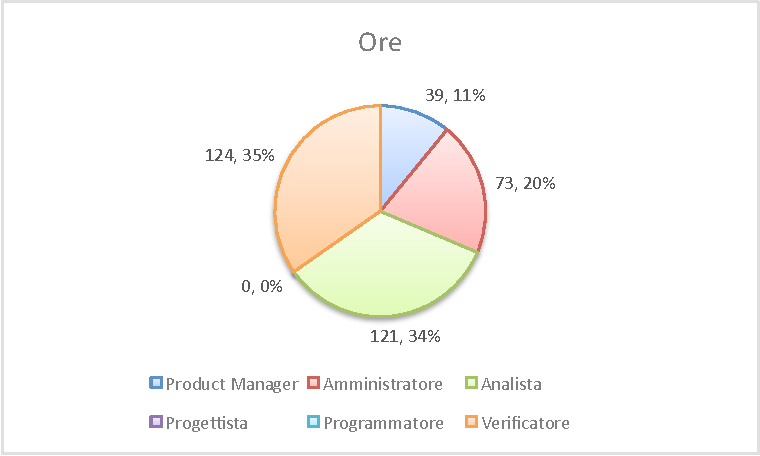
\includegraphics[width=\textwidth]{PianoDiProgetto/Pics/ChartTotOreInvest.pdf}
					\caption{Pie Chart ore di investimento}
				\end{figure}
				Riassumendo i costi per ruolo con un Pie Chart:
				\begin{figure}[H]\centering
					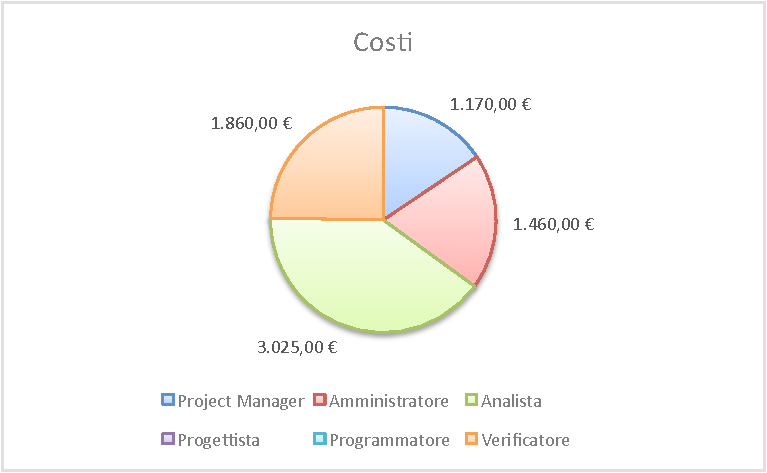
\includegraphics[width=\textwidth]{PianoDiProgetto/Pics/ChartTotCostiInvest.pdf}
					\caption{Pie Chart investimento per ruolo}
				\end{figure}
			\subsubsection{Conclusione}
				Il costo totale dell'investimento da parte del gruppo è di \euro{} 7~515,00 